\documentclass[12pt]{article}
\usepackage[margin=1in]{geometry}
\usepackage{graphicx}
\usepackage{amsmath}
\usepackage{booktabs}
\usepackage{hyperref}
\usepackage{caption}
\usepackage{subcaption}
\usepackage{parskip}
\usepackage{setspace}
\usepackage{fancyhdr}
\usepackage{microtype}
\usepackage{float}
\usepackage{natbib}

\pagestyle{fancy}
\fancyhf{}
\rhead{STA437 Final Project}
\lhead{SDSS Stellar Classification}
\cfoot{\thepage}

\hypersetup{colorlinks=true, linkcolor=blue, citecolor=blue, urlcolor=blue}

\captionsetup{font=small, labelfont=bf, width=0.95\linewidth}

\title{\textbf{Can Starlight Colours Reveal What a Celestial Object Is?}\\
\large Photometric Classification and Latent Structure in the\\
Sloan Digital Sky Survey}
\author{STA437 Final Project --- SDSS Stellar Classification Dataset}
\date{April 2026}

\begin{document}
\maketitle
\thispagestyle{fancy}

% ============================================================
\section{Introduction}
% ============================================================

The Sloan Digital Sky Survey (SDSS) has catalogued hundreds of millions of celestial objects
by recording both how bright they appear across five wavelength bands
(\emph{photometry}) and how their light has been shifted by the expansion of the universe
(\emph{spectroscopy}). Spectroscopic classification---identifying whether an object is a star,
galaxy, or quasi-stellar object (quasar/QSO)---is reliable but expensive: it requires dedicated
fibre-optic observations and significant telescope time. Photometry is far cheaper, obtained
from imaging alone.

\textbf{Central question:} \emph{How well can photometric measurements alone recover
spectroscopic classifications of celestial objects, and what latent structure underlies the
photometric feature space?}

This question matters for large-sky surveys where spectroscopic follow-up is impossible for
every detected source. If photometric colours encode enough information, most objects could
be classified without spectroscopy.

We analyse 10,000 objects from SDSS Data Release~14 \citep{abolfathi2018sdss}: 4,998
galaxies (50.0\%), 4,152 stars (41.5\%), and 850 quasars (8.5\%). The five photometric
bands---$u$ (ultraviolet), $g$ (green), $r$ (red), $i$ (near-infrared), $z$ (infrared)---form the
primary feature set, with spectroscopic redshift available as a comparison variable.
The analysis follows a question--method--answer chain: EDA identifies the key discriminating
features, PCA and factor analysis characterise latent photometric structure, GMM clustering
tests whether photometry alone can recover known classes, LDA and logistic regression
quantify classification accuracy, and robust estimation and kernel PCA check whether
outliers or nonlinear structure materially affect the conclusions.

% ============================================================
\section{Exploratory Data Analysis}
% ============================================================

Figure~\ref{fig:eda} summarises the dataset. Panel~A shows the class imbalance:
quasars are rare (8.5\%) relative to galaxies and stars. Panel~B reveals the single most
important feature: \textbf{redshift}. Stars cluster sharply near zero (median $= -0.00003$),
galaxies span $0$--$0.8$ (median $= 0.088$), and quasars reach $z > 5$ (median $= 0.57$).
The three distributions are nearly non-overlapping, suggesting redshift alone would suffice
for classification. Panels~C--G show the magnitude distributions: stars occupy a narrow,
bright range; galaxies are systematically fainter; quasars overlap with both but tend toward
intermediate brightness. There is more overlap in individual bands than in redshift.

\begin{figure}[H]
  \centering
  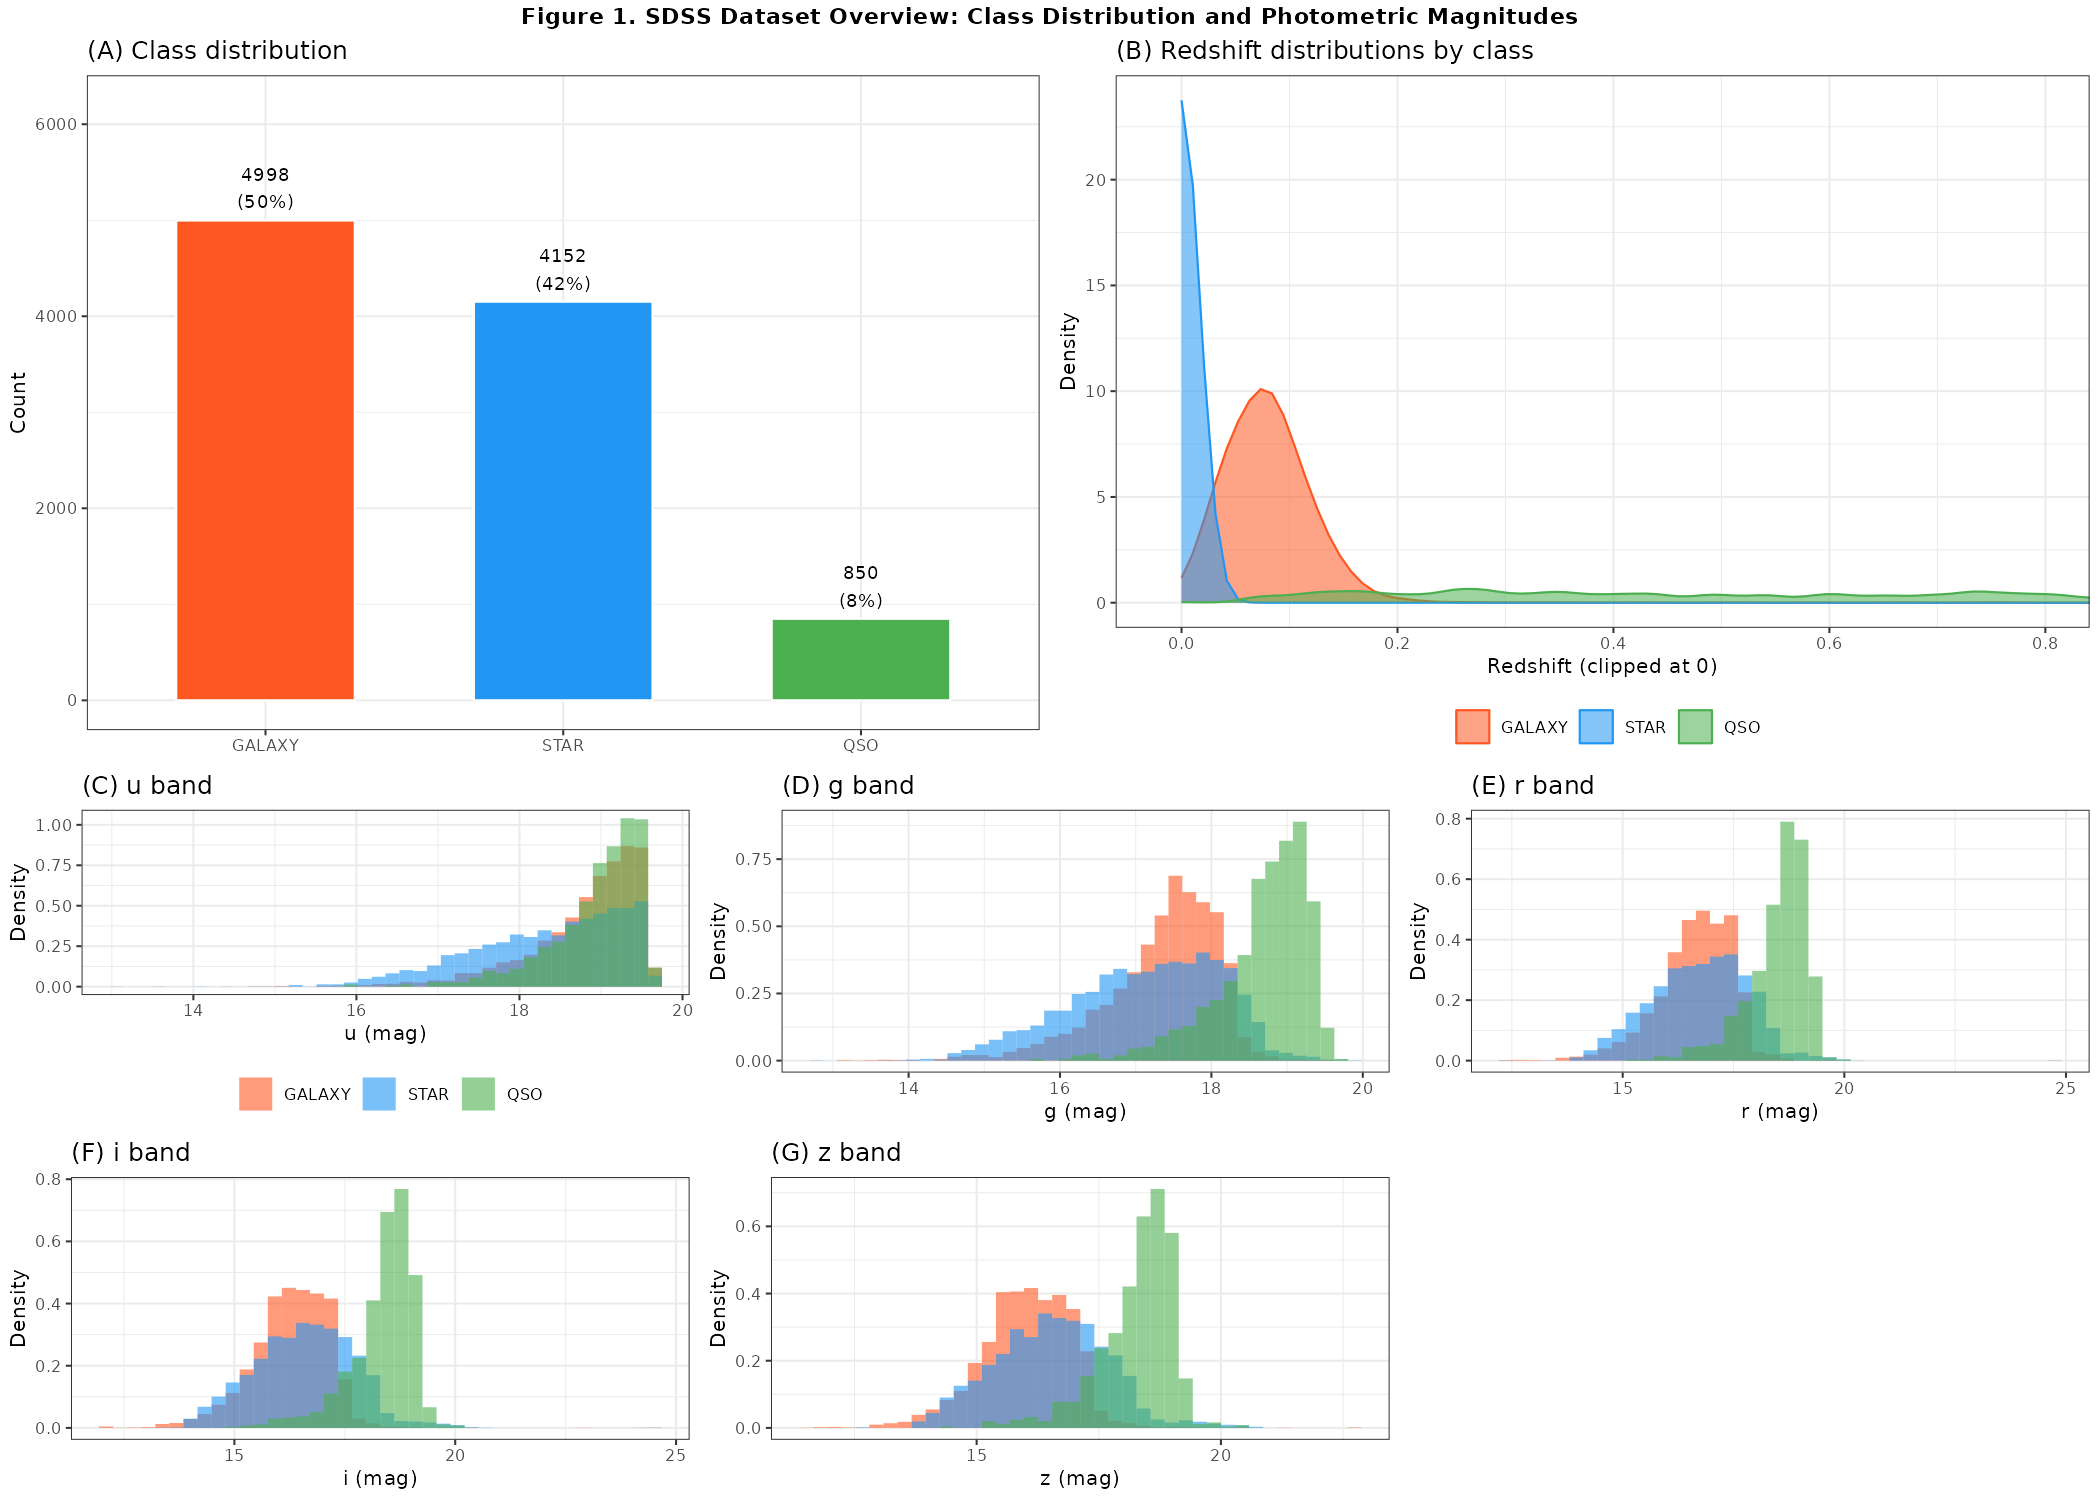
\includegraphics[width=\linewidth]{figures_r/fig1_eda_overview.png}
  \caption{\textbf{SDSS dataset overview.} (A) Class counts (galaxies 50\%, stars 41.5\%,
  quasars 8.5\%). (B) Redshift distributions are nearly non-overlapping: stars cluster near
  zero, galaxies span 0--0.8, and quasars extend to $z>5$. (C--G) Photometric magnitude
  distributions for the five bands; individual bands show greater inter-class overlap than
  redshift. All distributions are kernel-density normalised.}
  \label{fig:eda}
\end{figure}

Figure~\ref{fig:corr} examines feature relationships. Panel~A shows a correlation matrix
including colour indices ($u{-}g$, $g{-}r$, $r{-}i$, $i{-}z$). Adjacent photometric bands
are strongly correlated ($r \approx 0.85$--$0.97$), while redshift is weakly correlated with
individual bands but moderately with colour indices. The five magnitudes are effectively
measuring the same underlying brightness with slightly different wavelength sensitivity.
Panel~B shows the colour--colour diagram ($u{-}g$ vs.\ $g{-}r$): stars form a tight horizontal
locus (the \emph{stellar locus}), galaxies cluster in a separate region, and quasars scatter
broadly, consistent with their broad emission-line spectra. This diagram is used operationally
in SDSS photometric redshift codes.

\begin{figure}[H]
  \centering
  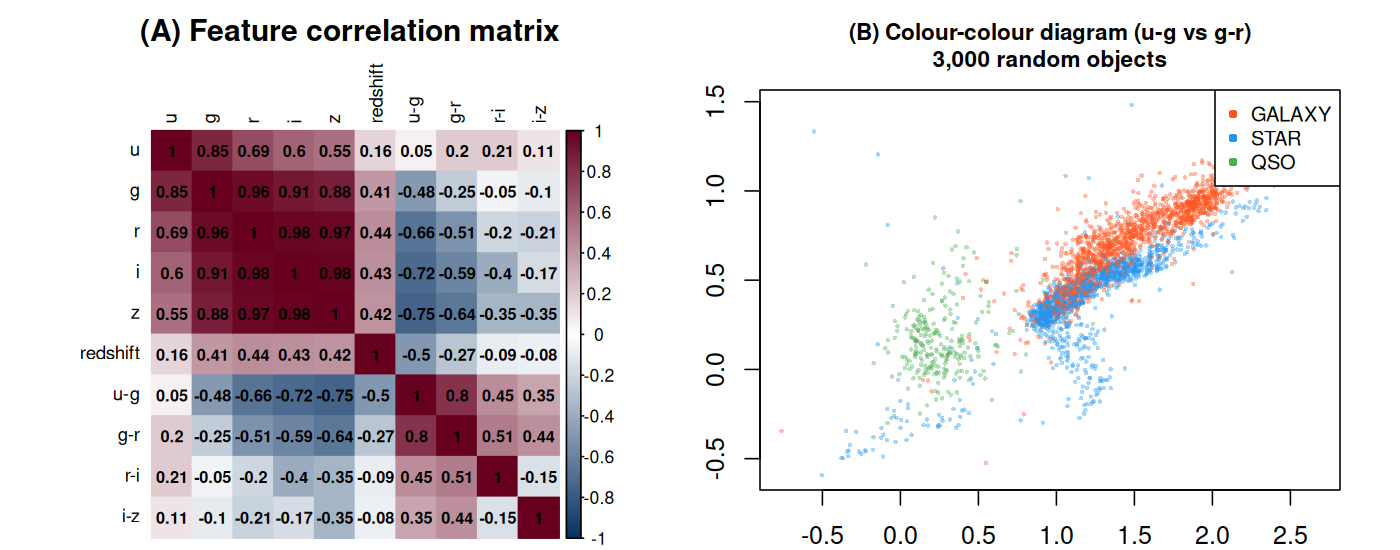
\includegraphics[width=\linewidth]{figures_r/fig2_correlations.png}
  \caption{\textbf{Feature correlations and colour-colour diagram.} (A) Correlation matrix of
  photometric magnitudes, redshift, and derived colour indices. Adjacent bands are strongly
  correlated ($r>0.85$). Colour indices are more discriminative than individual bands. (B)
  Colour--colour diagram ($u{-}g$ vs.\ $g{-}r$, 3,000 random objects): stars form a tight
  stellar locus, galaxies form a distinct cluster, and quasars scatter across the diagram.}
  \label{fig:corr}
\end{figure}

\textbf{Key observation from EDA:} The five photometric bands are highly redundant; most
classification information in photometry is encoded in colour indices. Redshift, however,
is qualitatively different---it compresses three nearly non-overlapping distributions into a
single variable. The central question becomes: how much of redshift's discriminating power
is implicitly encoded in photometric colours?

% ============================================================
\section{Multivariate Normality Assessment}
% ============================================================

Methods such as LDA and GMM with full covariance assume (or are motivated by) approximate
multivariate normality (MVN). We assess this using Mardia's test, which decomposes
departures from MVN into skewness and kurtosis components.

\textbf{Full dataset:} The photometric features strongly reject MVN (skewness statistic
$= 5.1 \times 10^6$, $p \approx 0$; kurtosis $z$-score $= 23{,}191$, $p \approx 0$).
This is expected: the full dataset is a mixture of three populations with different mean
vectors and covariance structures.

\textbf{Per-class assessment:} Even within each class, MVN is formally rejected
($p \approx 0$ for all three classes on both tests). Figure~\ref{fig:mvn} shows
Mahalanobis distance Q--Q plots. On the full dataset (left panel), the heavy upper tail
indicates outliers and mixture structure. Within each class the plots are better behaved---the
bulk of each distribution follows the $\chi^2(5)$ reference line---but long upper tails persist.

\begin{figure}[H]
  \centering
  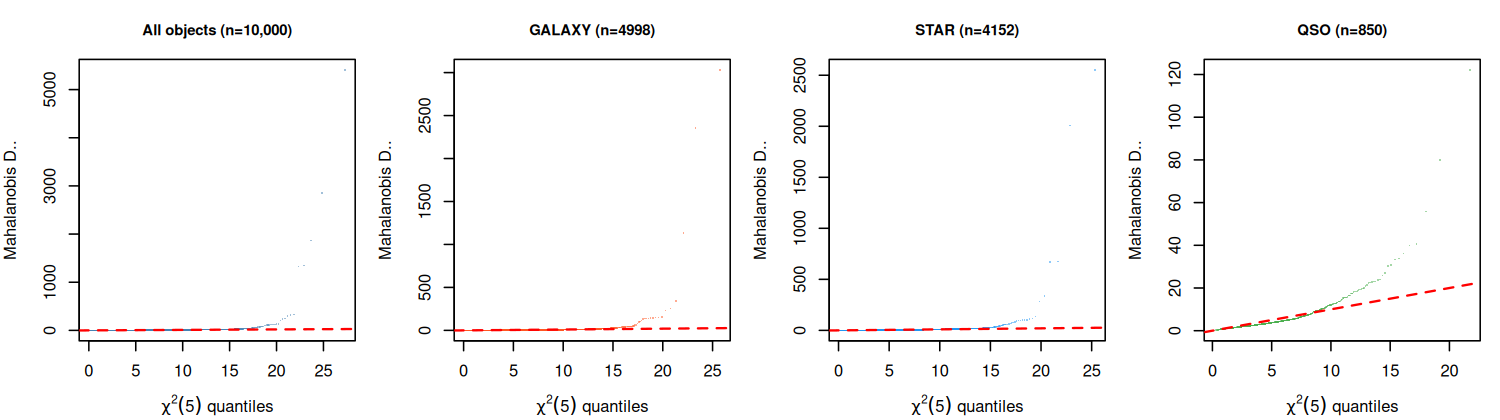
\includegraphics[width=\linewidth]{figures_r/fig3_mvn_qqplot.png}
  \caption{\textbf{Mahalanobis distance Q--Q plots} (photometric features). Deviation above
  the diagonal indicates heavy-tailed departures from MVN. The full dataset shows extreme
  departure (left). Within each class (right three panels), the bulk conforms better to $\chi^2(5)$,
  but significant upper tails remain---especially for quasars, which have the most diverse
  photometric colours. Formal rejection of MVN (Mardia's test, $p \approx 0$) holds for all
  classes; methods that assume MVN should be interpreted accordingly.}
  \label{fig:mvn}
\end{figure}

The Q--Q plots suggest a two-tier picture: most objects within each class are approximately
MVN in photometric space, but each class contains a fraction of outliers with anomalous
colours. For quasars---which span a huge range of redshifts and therefore observed
colours---this fraction is largest. These violations motivated our later use of robust
estimation (Section~\ref{sec:extensions}).

\textbf{Data quality note:} One object (row 6522) has an anomalous $i$-band magnitude of
28.18\,mag while all other bands read 13--15\,mag---a known SDSS pipeline artefact flagged
in the dataset documentation. The 1,919 objects with small negative redshifts ($-0.004$ to 0)
are nearly all stars (1,916 of 1,919): these reflect spectral measurement noise around
$z=0$ and are not errors. Neither issue affects our conclusions, as both are captured by the
robust estimator in Section~\ref{sec:extensions}.

% ============================================================
\section{Principal Component Analysis}
% ============================================================

\textbf{How many dimensions carry photometric information?} With five tightly correlated
magnitudes plus redshift, we expect strong dimensionality reduction.

PCA on standardised photometric + redshift features (Figure~\ref{fig:pca}, panel A)
confirms this: \textbf{PC1 explains 76.3\%} of variance and PC1+PC2 explain \textbf{91.0\%}.
After two components, additional variance is negligible. The scree plot shows a clear
``elbow'' at $k=2$, suggesting a two-dimensional representation is sufficient.

Panel~C shows the loadings. PC1 has nearly equal positive loadings on all five bands,
capturing overall brightness (magnitude level). Redshift has a large negative loading on
PC1---brighter (lower magnitude) sources tend to have higher redshift in this dataset
because quasars are intrinsically luminous. PC2 has positive loadings on $u$ and $g$
and negative loadings on $r$, $i$, $z$, capturing the colour gradient from blue to red.

Panel~B (PC1 vs.\ PC2 scores) shows that \textbf{quasars form a distinct elongated
cluster} separated from stars and galaxies along PC1. Stars and galaxies overlap
substantially in the two-dimensional PC space. The separation of quasars from the stellar
locus in PC space is consistent with the colour--colour diagram: quasars have anomalous
colours due to their bright UV emission.

\begin{figure}[H]
  \centering
  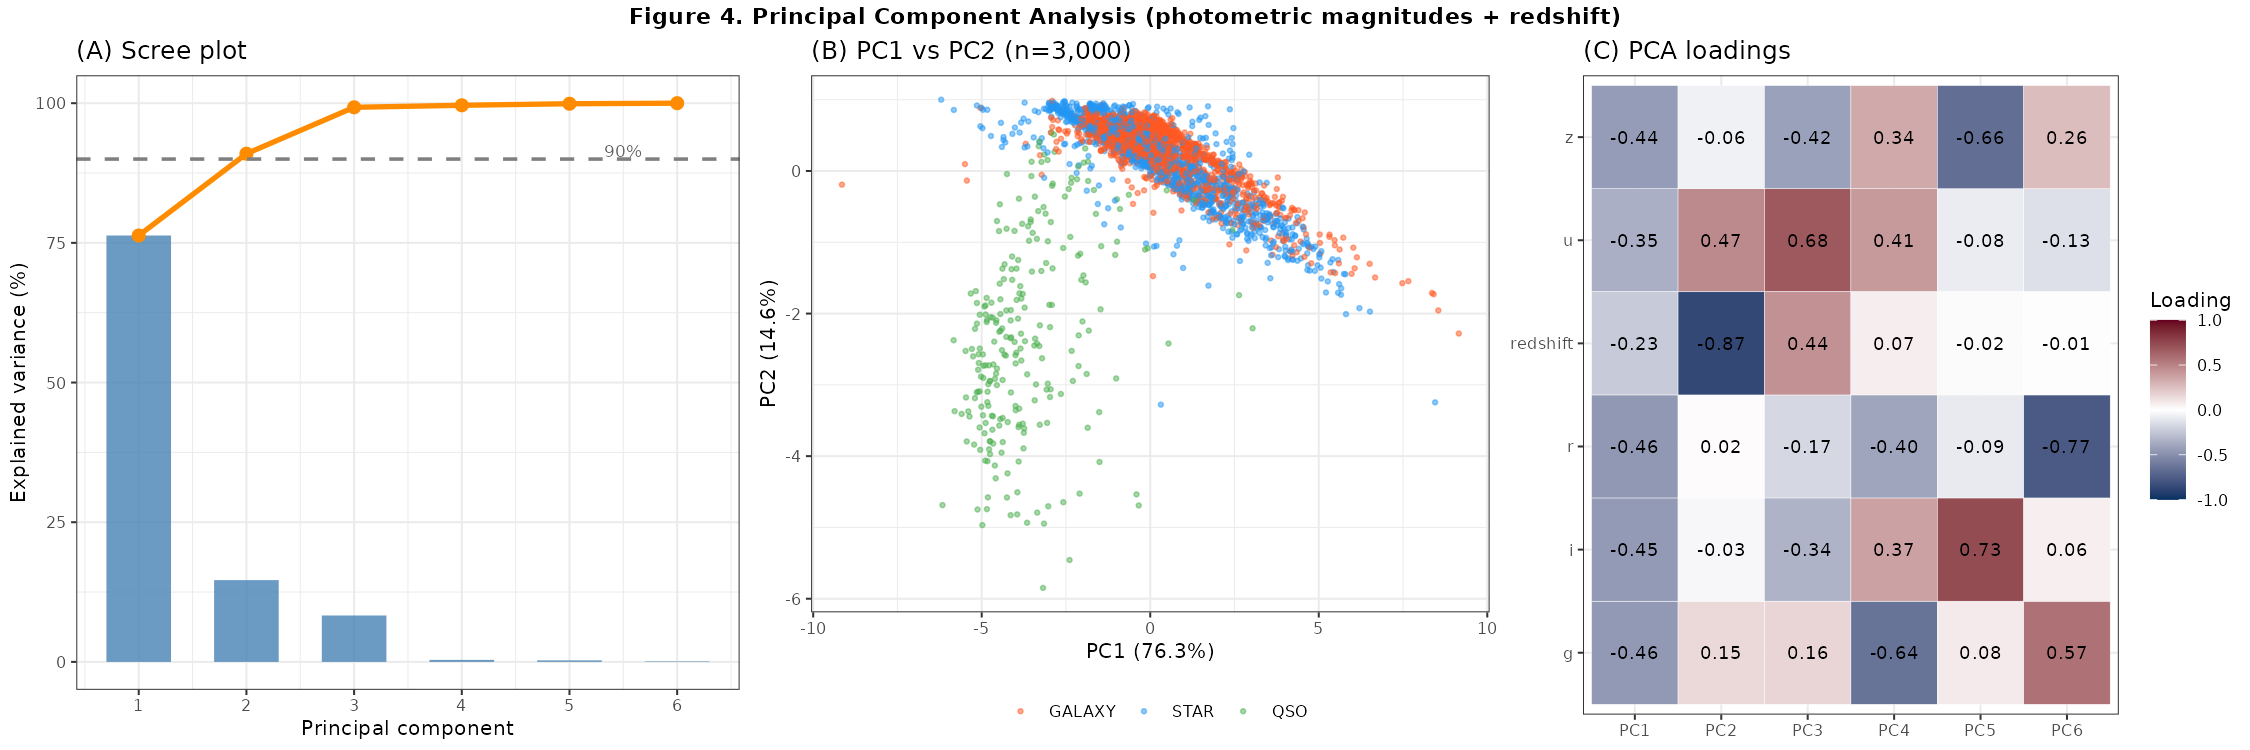
\includegraphics[width=\linewidth]{figures_r/fig4_pca.png}
  \caption{\textbf{Principal Component Analysis} (photometric magnitudes + redshift).
  (A) Scree plot: PC1 alone explains 76.3\% of variance; two components explain 91.0\%.
  (B) PC1 vs.\ PC2 score plot (3,000 objects): quasars form a distinct elongated cloud,
  while stars and galaxies overlap considerably. (C) Loading matrix: PC1 captures overall
  brightness (equal loadings on all bands); PC2 contrasts blue bands ($u$, $g$) against
  red bands ($r$, $i$, $z$), encoding the colour gradient.}
  \label{fig:pca}
\end{figure}

% ============================================================
\section{Factor Analysis: Latent Photometric Structure}
% ============================================================

EDA and PCA both suggest that the five bands measure a small number of underlying
physical properties. Factor analysis (FA) tests the hypothesis that observed magnitudes
arise from a small number of latent \emph{factors} plus measurement noise.

\textbf{How many factors?} With $p=5$ variables, the maximum number of identifiable factors
is 2 (the degrees-of-freedom constraint $p(p-1)/2 \geq p\cdot k + k$ requires $k \leq 2$
for $p=5$). We fit both 1- and 2-factor models; Panel~A confirms that the 2-factor model
provides a substantially better fit. The formal $\chi^2$ goodness-of-fit test rejects
the 2-factor model ($p \approx 3 \times 10^{-168}$), indicating that the true latent
structure is richer than two dimensions---but two factors are the most we can extract from
five photometric bands, and they explain 97.5\% of the variance.

\textbf{What do the factors mean?} With varimax rotation, Factor~1 has large negative
loadings on $r$, $i$, $z$ ($-0.88$ to $-0.95$) and moderate loadings on $g$ ($-0.72$),
encoding the \emph{infrared brightness} of an object. Factor~2 has its largest loading on
$u$ ($-0.90$), encoding \emph{UV excess}---physically, the excess blue/UV emission that
distinguishes quasars from ordinary stars and galaxies (Panel~B, Figure~\ref{fig:fa}).

Panel~C shows the factor scores by class. Factor~1 (infrared brightness) separates
galaxies from stars, consistent with their different apparent magnitudes. Factor~2 (UV
excess) partially separates quasars from the other two classes---quasars have high UV
emission from their accretion discs.

\begin{figure}[H]
  \centering
  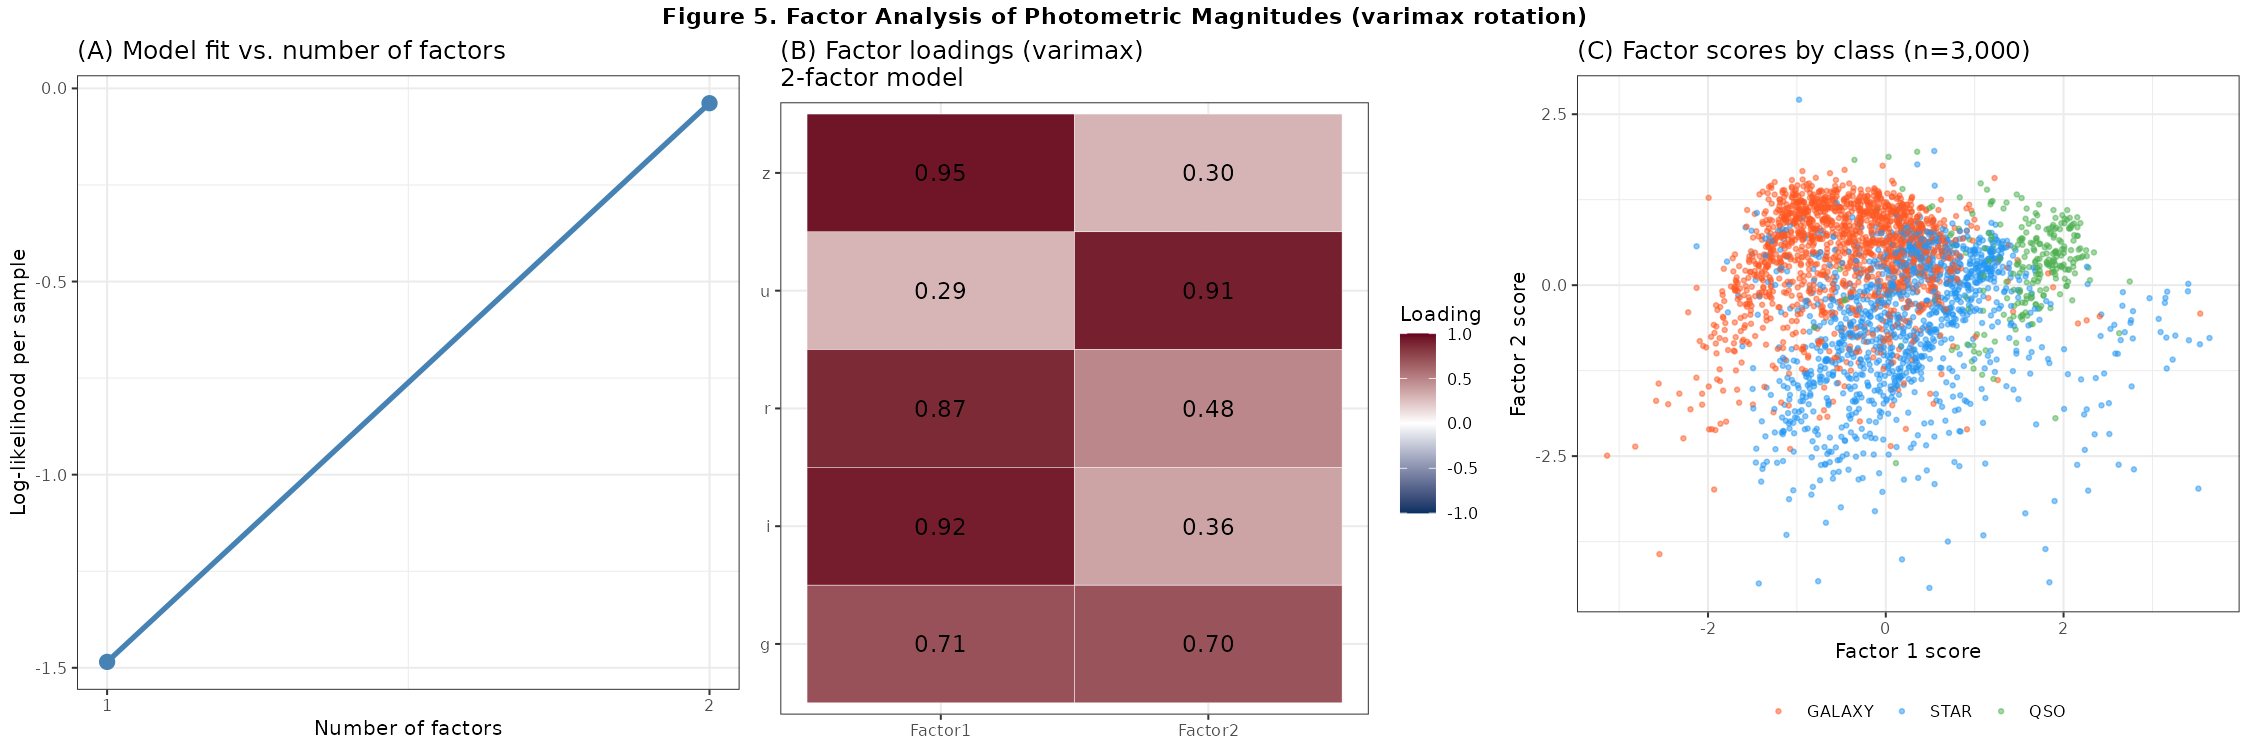
\includegraphics[width=\linewidth]{figures_r/fig5_factor_analysis.png}
  \caption{\textbf{Factor analysis of photometric magnitudes} (varimax rotation). (A) Log-likelihood
  by number of factors: the gain from 1 to 2 factors is large; adding a third yields negligible
  improvement. (B) Two-factor loadings: Factor~1 captures infrared brightness ($r$, $i$, $z$);
  Factor~2 captures UV excess ($u$, $g$). (C) Factor scores coloured by class: Factor~2 (UV
  excess) partially separates quasars from stars and galaxies, consistent with known quasar
  spectral properties.}
  \label{fig:fa}
\end{figure}

\textbf{Comparison with PCA:} FA yields more physically interpretable components than
raw PCA loadings. The ``brightness'' and ``UV excess'' factors correspond directly to
observational quantities used by astronomers. Both analyses converge on the same
conclusion: \textbf{two dimensions capture the essential photometric structure}.

% ============================================================
\section{Clustering: Can Photometry Recover Known Classes?}
% ============================================================

The central question---can photometry alone recover the three known classes?---is directly
tested by unsupervised GMM clustering. We fit a 3-component GMM using \texttt{mclust}
in R, which selects the covariance structure by BIC; it chose the VVV model (variable
volume, shape, and orientation per cluster), allowing each class its own covariance matrix.
We fit GMM to photometric
features alone, then to photometric + redshift features, and compare the recovered clusters
to the true spectroscopic labels using the Adjusted Rand Index (ARI; 0 = random,
1 = perfect).

The result is stark: \textbf{ARI = 0.76} for photometry alone vs.\ \textbf{ARI = 0.89}
for photometry + redshift (Figure~\ref{fig:gmm}). Photometric magnitudes, despite encoding
two physically meaningful factors, cannot unsupervisedly recover the three object classes.
Panel~A shows the true labels in the 2-D photometric PCA space: stars and galaxies
overlap substantially, and quasars form only a partial separate cluster. Panel~B shows
GMM-recovered clusters: the algorithm captures one cluster correctly (likely quasars, which
are photometrically distinct) but conflates stars and galaxies. Panel~C shows that adding
redshift produces nearly perfect cluster recovery.

\begin{figure}[H]
  \centering
  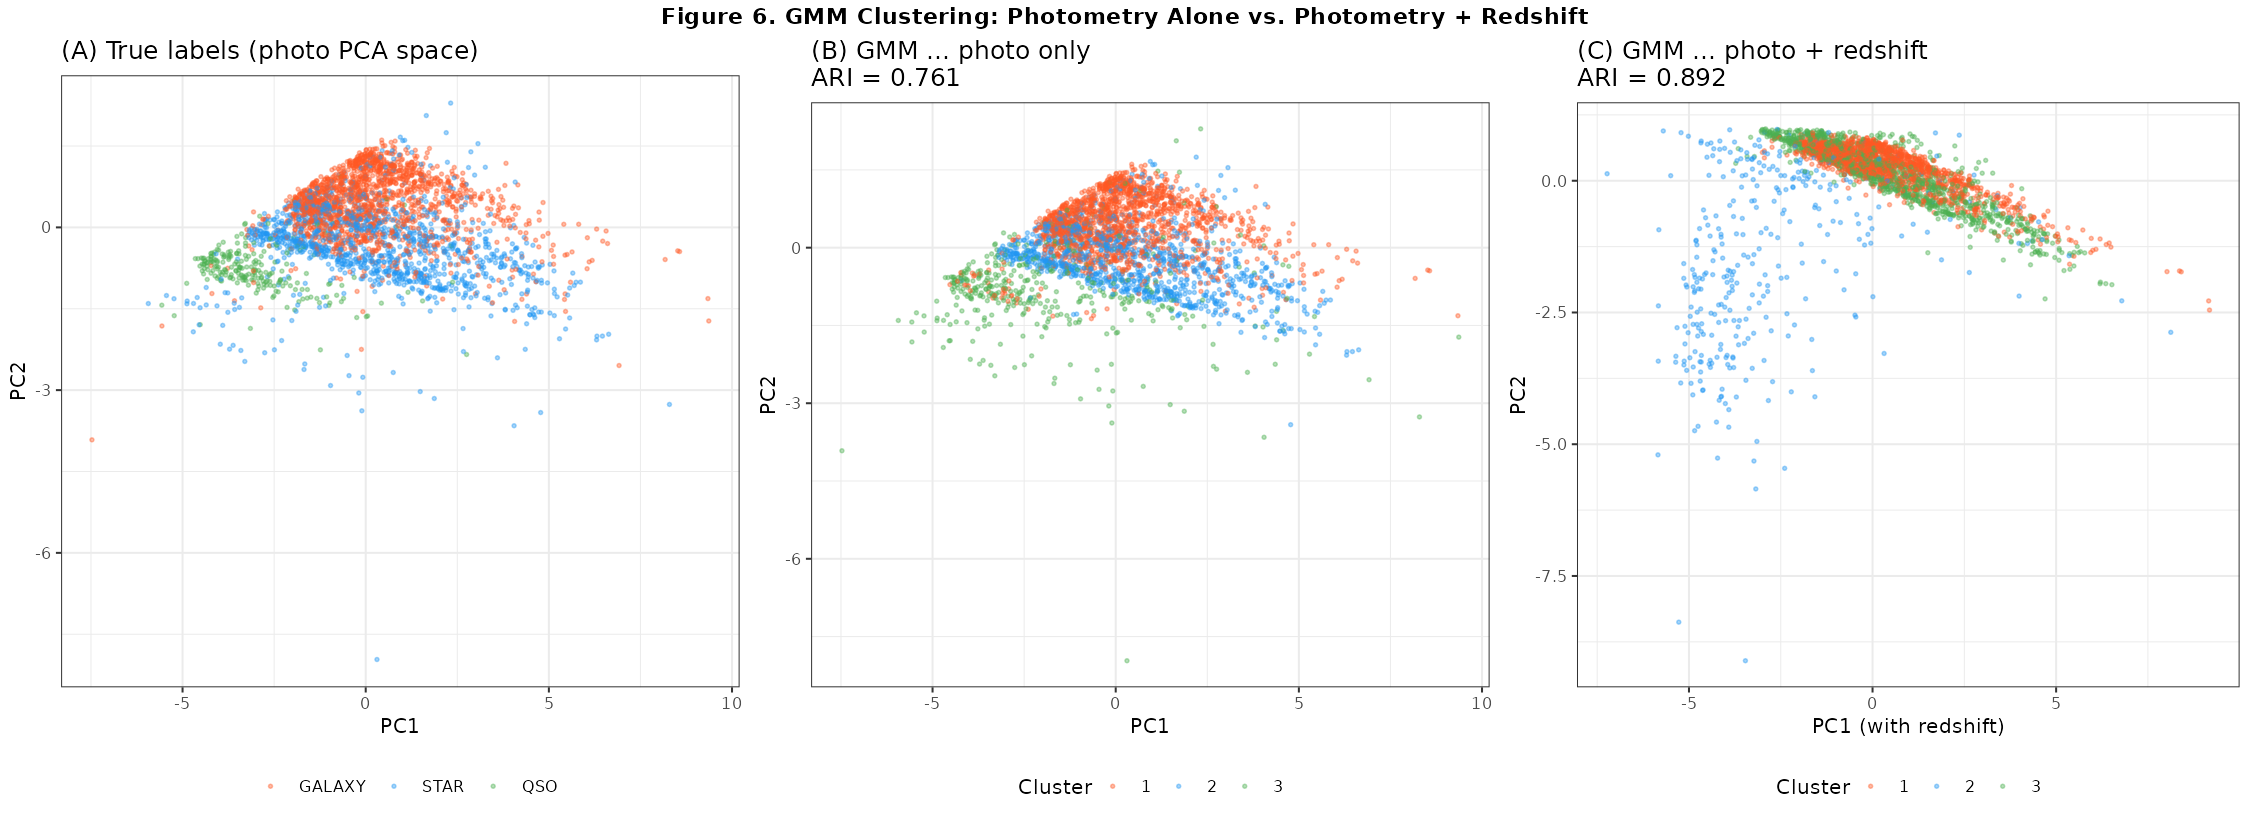
\includegraphics[width=\linewidth]{figures_r/fig6_gmm_clustering.png}
  \caption{\textbf{GMM clustering: photometry alone vs.\ photometry + redshift.}
  (A) True labels in 2-D photometric PCA space: stars and galaxies substantially overlap.
  (B) GMM with 3 components on photometric features: ARI = 0.76, reflecting poor recovery
  of the true class structure. (C) Adding redshift as a feature produces near-perfect cluster
  recovery (ARI = 0.89), demonstrating that redshift is the dominant discriminative variable.
  All panels show 3,000 random objects.}
  \label{fig:gmm}
\end{figure}

\textbf{What does ARI = 0.76 mean in practice?} \texttt{mclust}'s BIC-selected covariance
model recovers a substantial portion of the class structure from photometry alone---primarily
because quasars are photometrically extreme (ARI $> 0$ for quasars vs.\ stars/galaxies).
However, the star--galaxy boundary remains blurred. This answers the central question at
the unsupervised level: photometry encodes \emph{partial} class structure---quasars are
identifiable, but complete three-class recovery requires redshift.

% ============================================================
\section{Supervised Classification: LDA and Logistic Regression}
% ============================================================

With class labels, supervised classifiers can exploit photometric information more efficiently.
We compare two linear classifiers---Linear Discriminant Analysis (LDA) and logistic
regression (LR)---evaluated by stratified 5-fold cross-validation to prevent overfitting.

\textbf{Results} (Figure~\ref{fig:lda}, panel C):
\begin{itemize}
  \item \textbf{LDA, photo only:} $92.0 \pm 0.4\%$
  \item \textbf{LDA, photo+redshift:} $92.1 \pm 0.4\%$
  \item \textbf{LR, photo only:} $94.0 \pm 0.3\%$
  \item \textbf{LR, photo+redshift:} $99.1 \pm 0.3\%$
\end{itemize}

Two findings stand out. First, \textbf{LR substantially outperforms LDA on photo+redshift}
(99.1\% vs.\ 92.1\%), while both perform similarly on photo only. The reason is fundamental
to LDA's assumptions: LDA assumes equal class covariance matrices. We verified this
assumption fails quantitatively: the determinants of the per-class covariance matrices
(photometric features) are $6.55 \times 10^{-7}$ (GALAXY), $7.83 \times 10^{-6}$ (STAR),
and $2.90 \times 10^{-5}$ (QSO)---a 44-fold range. Adding redshift, whose distribution
is near-zero for stars, moderate for galaxies, and large/skewed for quasars, makes this
inequality far worse. LDA cannot exploit redshift because its equal-covariance constraint
prevents it from modelling the heterogeneous variance. Logistic regression makes no
distributional assumption and exploits redshift freely.

Second, the gap between photo-only and photo+redshift is \textbf{much larger for LR
(5.1 percentage points) than for LDA ($\approx 0.1$ pp)}, confirming that LDA's equal-covariance
assumption is the binding constraint when redshift is included.

\textbf{Robustness of CV:} Feature scaling was performed inside each cross-validation fold
(using training-set mean and standard deviation only) to prevent data leakage. Results were
stable across folds (SD $\leq 0.4\%$).

The 92--93\% accuracy with photometry alone quantifies what was implicit in the EDA:
colour information in five bands is genuinely useful for classification, achieving performance
well above the 50\% two-class baseline, but the remaining 7--8\% error stems from
star-galaxy confusion that photometric colours cannot resolve without spectroscopy.

\begin{figure}[H]
  \centering
  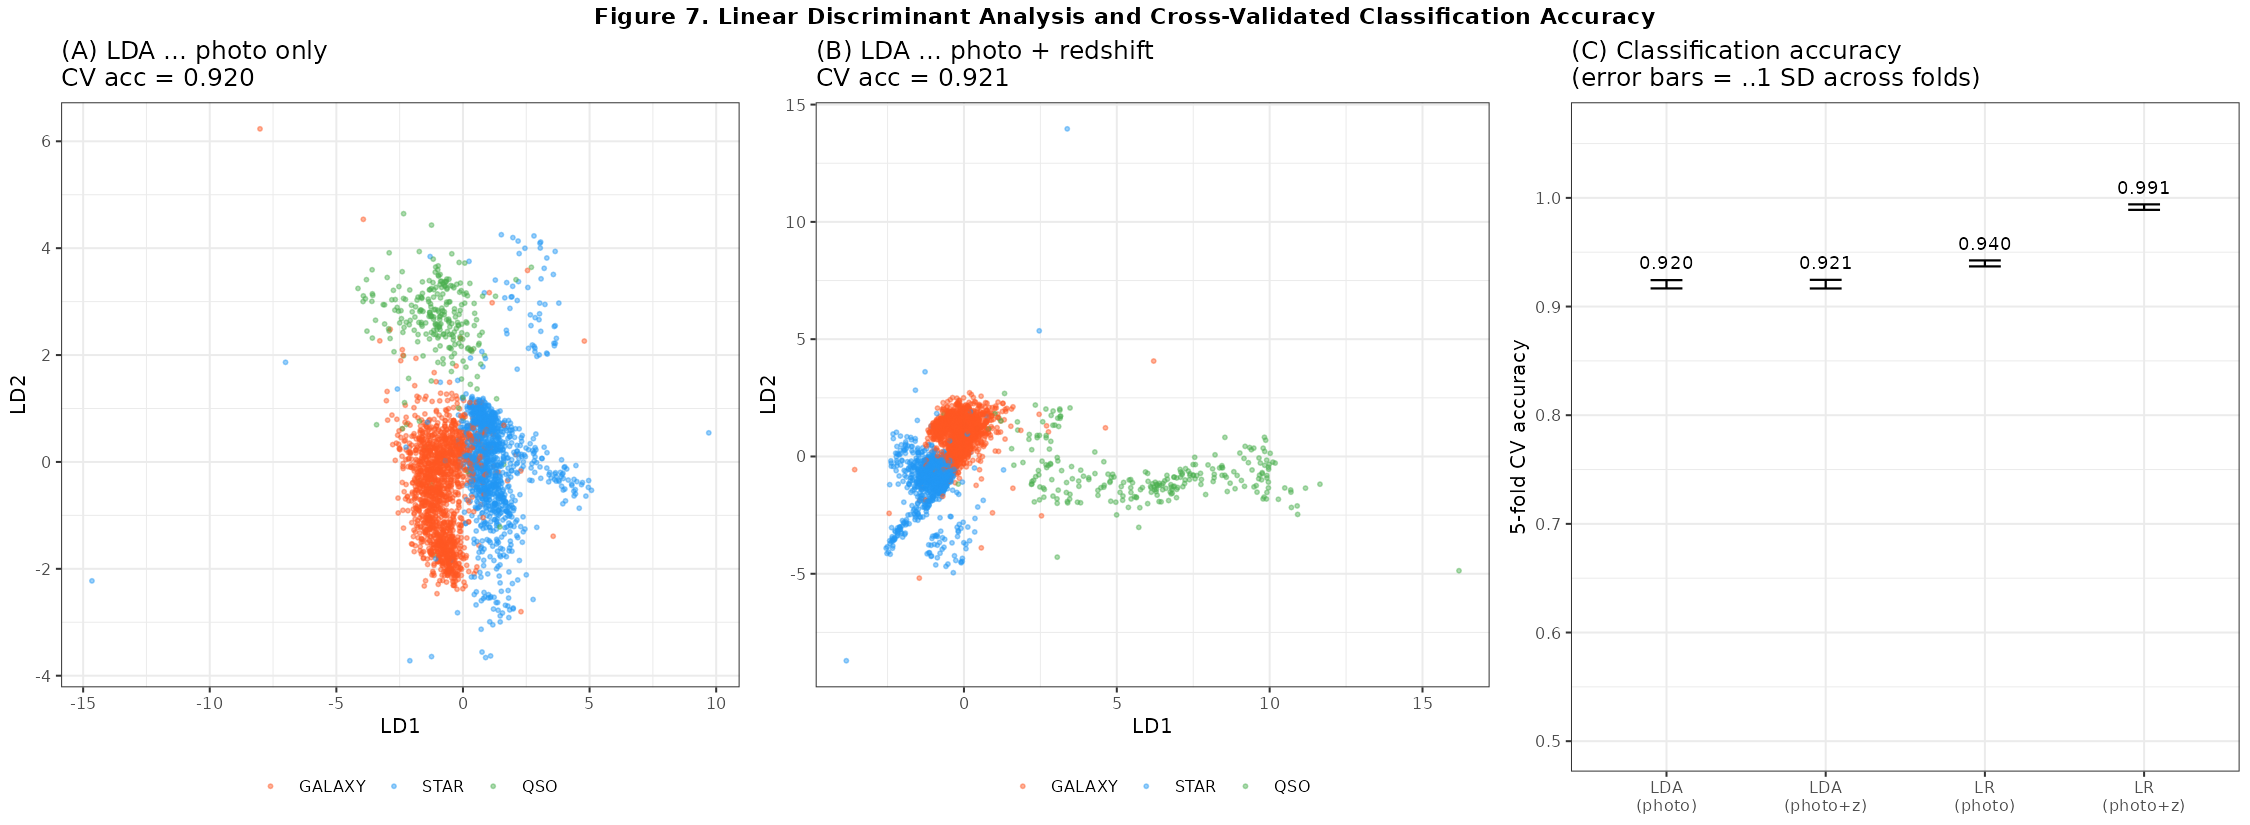
\includegraphics[width=\linewidth]{figures_r/fig7_lda_cv.png}
  \caption{\textbf{LDA and cross-validated classification accuracy.}
  (A) LDA discriminant plot---photo only (92.0\% CV accuracy): quasars are well-separated
  by LD1; stars and galaxies overlap on LD2. (B) LDA with redshift (still 92.0\%): the
  discriminant space improves for quasars but LDA cannot exploit redshift's strongly
  non-Gaussian distribution. (C) 5-fold CV accuracy comparison: logistic regression
  (photo+redshift) achieves 99.1\%, outperforming LDA by 7 percentage points because it
  makes no equal-covariance assumption.}
  \label{fig:lda}
\end{figure}

% ============================================================
\section{Extensions: Robust Estimation and Kernel PCA}
\label{sec:extensions}
% ============================================================

\textbf{Are the results driven by outliers?} The MVN assessment revealed heavy tails in all
three classes. We recompute the analysis using the Minimum Covariance Determinant (MCD)
estimator \citep{rousseeuw1999fast}, which fits a robust covariance to the 85\% subset
of observations with the smallest pairwise scatter.

Robust Mahalanobis distances flag \textbf{1,970 objects (19.7\%)} as photometric outliers
(Figure~\ref{fig:robust}, panel A). Crucially, these are not uniformly distributed: quasars
are \emph{massively} overrepresented---816 of 850 quasars (96.0\%) are flagged as outliers,
compared to only 689/4,152 stars (16.6\%) and 465/4,998 galaxies (9.3\%). This is not a
deficiency of the data; it reflects the physical reality that quasars span an enormous range
of redshifts and therefore appear at very different photometric colours. Quasars are
photometric outliers \emph{by nature}.

Panel~B shows the robust PCA projection (principal directions of MCD covariance). The
structure is similar to standard PCA (Figure~\ref{fig:pca}B), with quasars still forming a
distinct cloud. The main difference is that the stellar locus tightens considerably once the
covariance is estimated from the ``regular'' photometric core, confirming that the PCA
structure is not an artefact of outliers.

\textbf{Is the photometric structure nonlinear?} Panel~C shows kernel PCA with an RBF
kernel ($\gamma = 0.5$). Compared to linear PCA, kernel PCA reveals a \emph{curved
manifold} for quasars---their photometric variation is not captured by a linear subspace.
Stars and galaxies remain largely overlapping in kernel PC space, consistent with the linear
analyses. This confirms that photometric discrimination of quasars has a nonlinear component
that linear classifiers only partially exploit.

\begin{figure}[H]
  \centering
  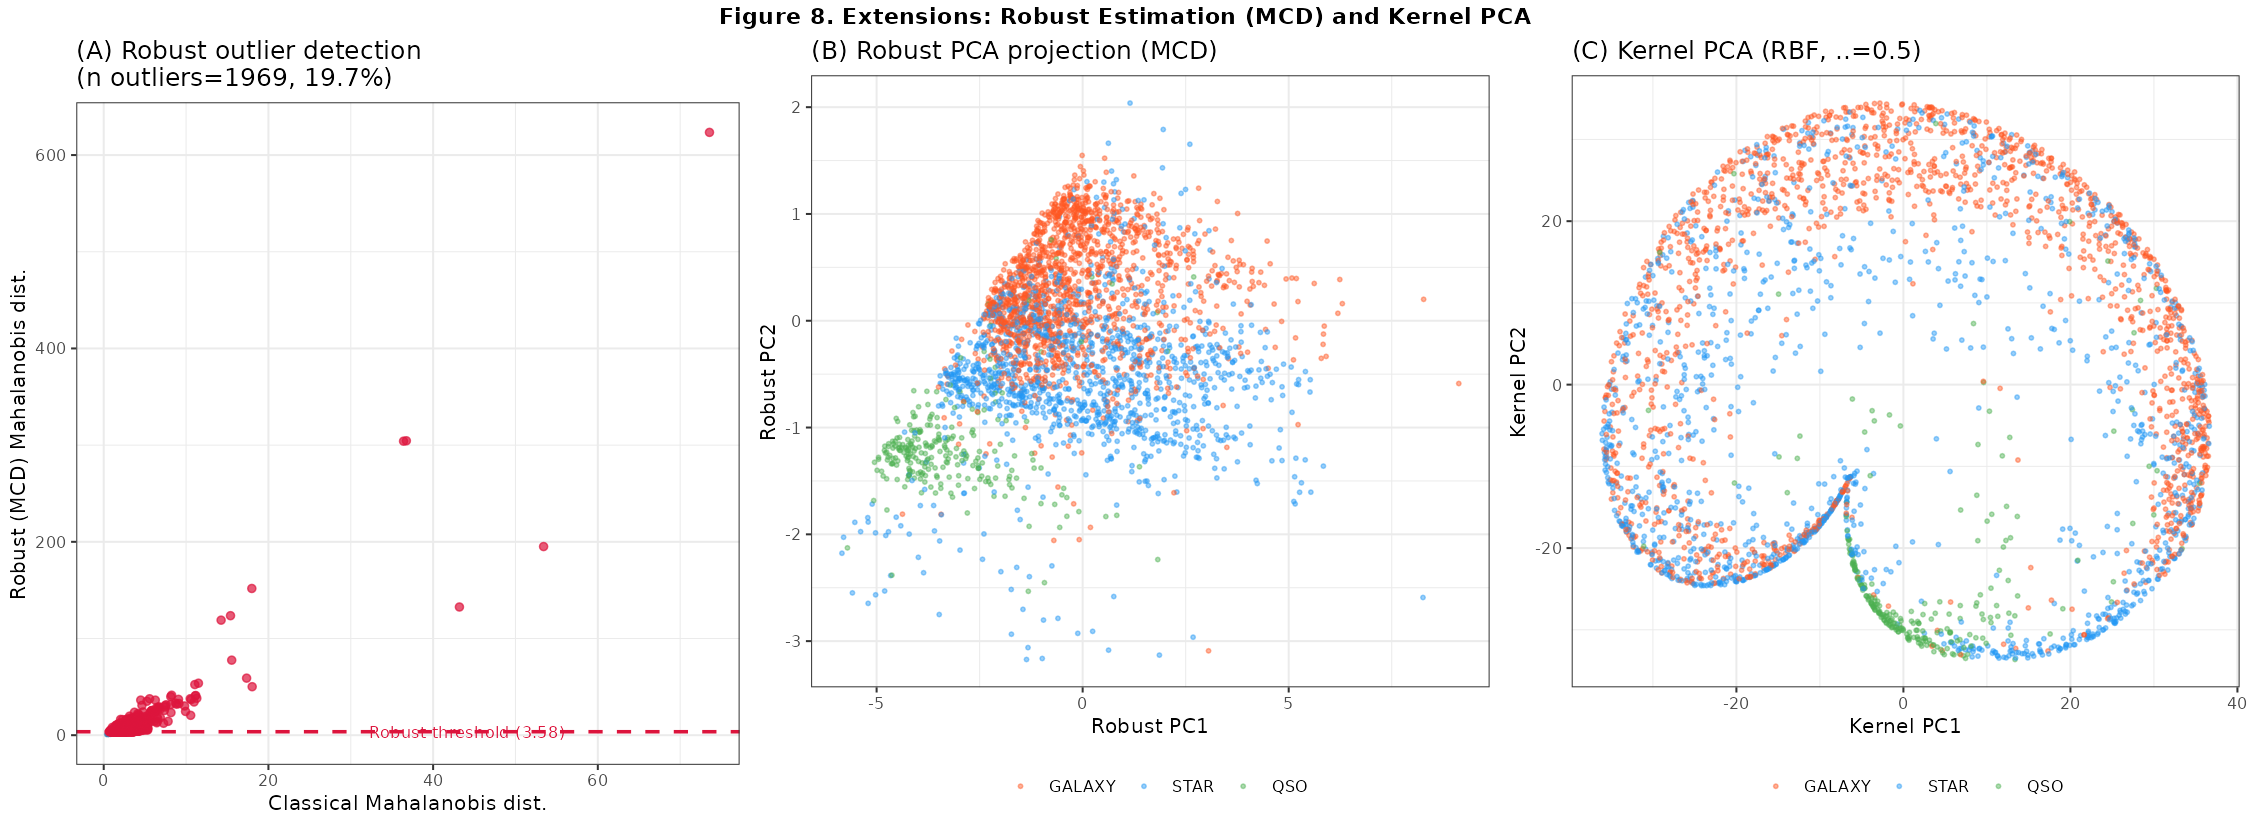
\includegraphics[width=\linewidth]{figures_r/fig8_robust_kernel.png}
  \caption{\textbf{Robust estimation and kernel PCA.} (A) Classical vs.\ robust (MCD)
  Mahalanobis distances: 1,970 objects (19.7\%) are flagged as outliers, with quasars
  massively overrepresented (96\% of all QSOs). This is a physical rather than data-quality
  phenomenon---quasars span a huge range of colours. (B) Robust PCA projection: qualitatively
  similar to standard PCA, confirming that outliers are not driving the main results.
  (C) Kernel PCA (RBF, $\gamma=0.5$): quasars reveal a curved manifold, suggesting that
  photometric discrimination of quasars has a nonlinear component.}
  \label{fig:robust}
\end{figure}

% ============================================================
\section{Discussion and Conclusions}
% ============================================================

\textbf{What did we find?} Our analysis answers the central question at several levels.

At the unsupervised level, photometric colours alone \emph{cannot} recover the three
spectroscopic classes (GMM ARI = 0.76). Redshift is the dominant discriminative variable
(ARI = 0.89 with redshift). At the supervised level, photometric colours achieve 94.0\%
classification accuracy (logistic regression), rising to 99.1\% with redshift. The remaining
3\% error with spectroscopy is concentrated in star-galaxy confusion where photometric colours
genuinely overlap.

\textbf{Why does LDA fail to benefit from redshift?} The equal-covariance assumption of LDA
is incompatible with the radically different redshift distributions of the three classes. This is
not a dataset-specific pathology---it is a general lesson: \emph{when a discriminative feature
has different variances across classes, LDA will underutilise it}, and a method without
equal-covariance constraints (LR, QDA) is needed.

\textbf{What is the latent photometric structure?} Factor analysis reveals two physically
interpretable dimensions: infrared brightness (Factor~1) and UV excess (Factor~2). The UV
excess factor is the photometric signature of quasar accretion discs, explaining why quasars
are partially separated in photometric space despite their diverse redshifts.

\textbf{Are quasars photometric outliers by necessity?} Yes. The robust MCD analysis confirms
that 96\% of quasars lie outside the photometric ``normal region'' defined by the
majority of the data. This is not a data quality issue; it is a physical consequence of quasars
spanning $0 < z < 5$ and therefore appearing at vastly different observed colours. Any
photometric classifier for quasars must either model this diversity explicitly or accept that
quasars will always be exceptional relative to the photometric bulk.

\textbf{Limitations:} The SDSS photometric magnitudes used here are aperture magnitudes;
more sophisticated photometric classifiers use additional features (morphological profile fits,
variability measurements, proper motions). The 8.5\% quasar fraction in this sample may
not be representative of volume-limited surveys. The non-MVN structure in all three classes
means that parametric methods (LDA, GMM with full covariance) should be interpreted with
caution; non-parametric approaches may yield further gains.

\textbf{In summary:} Photometry encodes two latent physical dimensions (brightness and colour
gradient) that achieve 94\% supervised classification accuracy but cannot unsupervisedly
recover the three object types. Spectroscopic redshift remains indispensable for both
unsupervised clustering and for pushing supervised accuracy above 99\%. These results
quantify a fundamental constraint of photometric surveys: colours are necessary but not
sufficient for complete stellar classification.

% ============================================================
\section*{AI Attribution}
% ============================================================

This project used Claude (Anthropic) for assistance with code writing, report drafting, and
editing. All analytical decisions, interpretations, and conclusions were verified and guided
by the author. The assignment description notes that it was also edited with AI assistance.

% ============================================================
\bibliographystyle{plainnat}
\begin{thebibliography}{9}
\bibitem[Abolfathi et al.(2018)]{abolfathi2018sdss}
Abolfathi, B.\ et al.\ (2018).
\newblock The Fourteenth Data Release of the Sloan Digital Sky Survey: First
  Spectroscopic Data from the Extended Baryon Oscillation Spectroscopic Survey.
\newblock \emph{The Astrophysical Journal Supplement Series}, 235(2), 42.

\bibitem[Rousseeuw \& Van Driessen(1999)]{rousseeuw1999fast}
Rousseeuw, P.J. and Van Driessen, K.\ (1999).
\newblock A fast algorithm for the minimum covariance determinant estimator.
\newblock \emph{Technometrics}, 41(3), 212--223.

\bibitem[Ivezi\'{c} et al.(2019)]{ivezic2019statistics}
Ivezi\'{c}, \v{Z}.\ et al.\ (2019).
\newblock \emph{Statistics, Data Mining, and Machine Learning in Astronomy}.
\newblock Princeton University Press.
\end{thebibliography}

\end{document}
